\documentclass{article}
\usepackage{amsmath}
\usepackage{amssymb}
\usepackage{graphicx}
\usepackage{hyperref}
\usepackage[version=4]{mhchem}


\begin{document}
\section*{Problem}
(1994 China Middle School Math Contest) \(\triangle A B C\) is an acute triangle. Three altitudes \(A D, B E, C F\) meet at point \(H . C\). If \(B C=a, A C=b, A B=c\), then the value of \(A H \cdot A D\) \(+B H \cdot B E+C H \cdot C F\) is\\
(A) \(\frac{1}{2}(a b+b c+c a)\)\\
(B) \(\frac{1}{2}\left(a^{2}+b^{2}+c^{2}\right)\)\\
(C) \(\frac{3}{2}(a b+b c+c a)\)\\
(D) \(\frac{3}{2}\left(a^{2}+b^{2}+c^{2}\right)\)\\
\centering
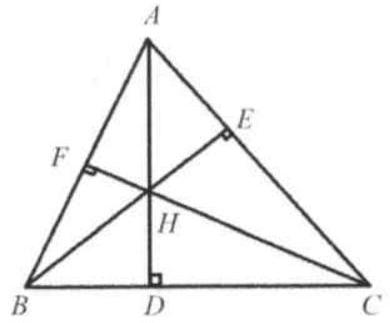
\includegraphics[width=\textwidth]{images/207(1).jpg}

\section*{Solution}
(B).\\
We know that points \(H, D, C\), and \(E\) are concyclic (Figure 1).\\
\centering
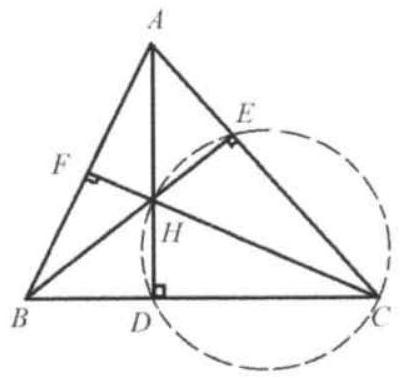
\includegraphics[width=\textwidth]{images/210(4).jpg}

Figure 1\\
\centering
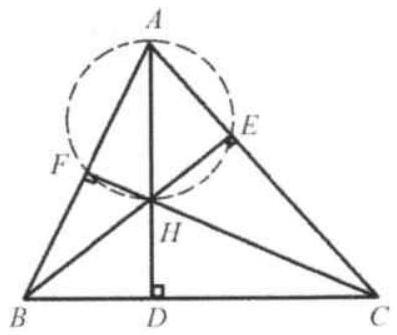
\includegraphics[width=\textwidth]{images/210(3).jpg}

Figure 2\\
\centering
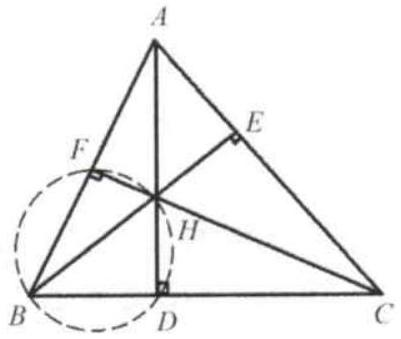
\includegraphics[width=\textwidth]{images/210(1).jpg}

Figure 3

So we have\\
\(A H \cdot A D=A E \cdot A C=A C \cdot A B \cdot \cos \angle B A E\)


By the law of cosine, \(\cos \angle B A E=\frac{A B^{2}+A C^{2}-B C^{2}}{2 A B \cdot A C}\). So\\
\(A H \cdot A D=\frac{1}{2}\left(A C^{2}+A B^{2}-B C^{2}\right)=\frac{1}{2}\left(b^{2}+c^{2}-a^{2}\right)\)\\
Similarly we have:\\
\(B H \cdot B E=B F \cdot B A=B A \cdot B C \cdot \cos \angle C B F\)\\
\(=\frac{1}{2}\left(A B^{2}+B C^{2}-A C^{2}\right)=\frac{1}{2}\left(c^{2}+a^{2}-b^{2}\right)\)\\
\(C H \cdot C F=C D \cdot C B=C B \cdot A C \cdot \cos \angle A C D\)\\
\(=\frac{1}{2}\left(A C^{2}+B C^{2}-A B^{2}\right)=\frac{1}{2}\left(b^{2}+a^{2}-c^{2}\right)\)\\
\((1)+(2)+(3): A H \cdot A D+B H \cdot B E+C H \cdot C F=\frac{1}{2}\left(a^{2}+b^{2}+c^{2}\right)\).\\
The answer is (B).

\end{document}
